\documentclass{kththesis}

\usepackage{blindtext} % This is just to get some nonsense text in this template, can be safely removed

\usepackage{csquotes} % Recommended by biblatex
\usepackage{biblatex}
\addbibresource{references.bib} % The file containing our references, in BibTeX format

%added by me:
\usepackage{xcolor}
\usepackage{color}
\usepackage{amsmath,float}
\usepackage{amssymb}
\usepackage{caption}
\captionsetup[figure]{labelfont=bf}
\usepackage{amsthm}
\theoremstyle{definition}
\newtheorem{definition}{Definition}[section]
\newtheorem{hyp}{Hypothesis}
\newtheorem{RQ}{Research Question}[section]
\newcommand\numberthis{\addtocounter{equation}{1}\tag{\theequation}}

\usepackage{graphicx}
\usepackage[]{algorithm2e} %for algos

%for clickable hyperlinks
%colors for different links
\usepackage{hyperref}
\hypersetup{
    colorlinks,
    linkcolor={red!50!black},
    citecolor={blue!50!black},
    urlcolor={blue!80!black}
}

\usepackage{cleveref}

\graphicspath{{Imgs/}}

\title{Competitive self-playing reinforcement learning agents used in the Nordic stock market, to understand market microstructure}

\alttitle{Reinforcement learning agenter i den nordiska aktiemarknaden, för att förstå marknadens mikrostruktur }
\author{Marcus Elwin}
\email{elwi@kth.se}
\supervisor{Hamid Reza Faragardi}
\examiner{Elena Troubitsyna}
\programme{Master of Science in Machine Learning}
\school{School of Electrical Engineering and Computer Science}
\date{\today}



\begin{document}


% Frontmatter includes the titlepage, abstracts and table-of-contents
\frontmatter

\titlepage

\begin{abstract}
  English abstract goes here.

\end{abstract}


\begin{otherlanguage}{swedish}
  \begin{abstract}
    Svensk sammanfattning
  \end{abstract}
\end{otherlanguage}


\tableofcontents


% Mainmatter is where the actual contents of the thesis goes
\mainmatter


\chapter{Introduction}

%We use the \emph{biblatex} package to handle our references.  We therefore use the
%command \texttt{parencite} to get a reference in parenthesis, like this
%\parencite{heisenberg2015}.  It is also possible to include the author
%as part of the sentence using \texttt{textcite}, like talking about
%the work of \textcite{einstein2016}.

\section{Background}
Modern financial markets such as NASDAQ, CME and NYSE have all been effected by the rise and presence of \textit{Algorithmic Trading} and \textit{High-Frequency Trading} (HFT).  Where both types of trading consists in using computer programs to implement investment and trading strategies \parencite{abergel2012market}. These types of strategies have according to \textcite{abergel2012market, o2015high} raised various questions about there effects on the financial markets. Mainly in areas as: \textit{liquidity, volatility, price discovery, systematic risk, manipulation} and \textit{market organization}. Where a quite recent example of the proposed effect of algorithmic trading and HFT on financial markets is \textit{the Flash Crash} in the 6th of May 2010. Where in the course of 30 minutes U.S. stock market indices, stock-index futures, options, and exchange-traded funds. Experienced a sudden price drop of more than five percent,followed by a rapid rebound \parencite{kirilenko2011flash,kirilenko2017flash}. See an illustration of this in \autoref{fig:1}.
\newline
\newline
Trading in the financial market can be seen as a search problem where buyers and sellers search for each-other. Which depends on market structure \parencite{abergel2012market}. \textit{Market microstructure} is a branch of economics, where one tries to understand trading dynamics on the financial market on a micro level \parencite{o1995market, hasbrouck2007empirical}. Market microstructure theory is used by regulators, traders and organizers of financial markets. In order to make a profit or create more transparent and efficient markets. Where a recent regulation with the purpose of making markets more transparent and efficient is \textit{Markets in Financial Instruments Directive} (MiFID) II \parencite{busch2016mifid}.

\begin{figure}[ht]
    \centering
    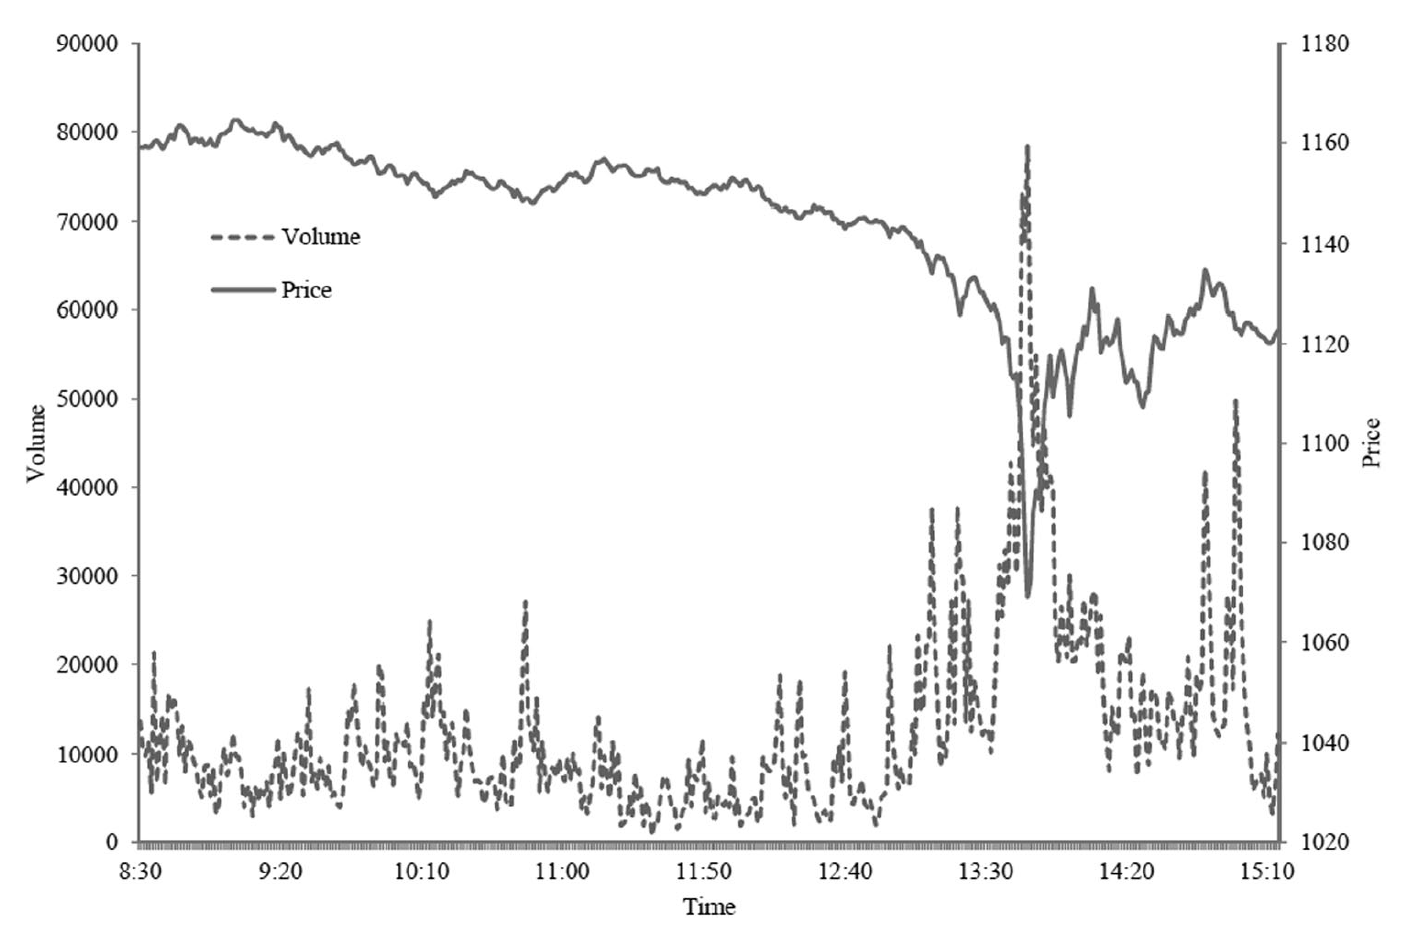
\includegraphics[scale=.7]{flashcrash.PNG}
    \caption{Minute-by-minute transaction prices and trading volume on E-mini S\& P futures contracts during the flash crash, between 8:30 to 15:15. Notice the distinct drop and rebound at the end of the day. Source: \textcite{kirilenko2017flash} }
    \label{fig:1}
\end{figure}

However as mentioned by \textcite{o2015high} due to HFT and algoritmic trading. Learning models and empirical models used in market microstructure in the past are deficient and may not longer be appropriate. Which calls for the use of new more capable methods. Where \textit{Reinforcement Learning} and other machine learning methods are of great interest. Machine learning and AI has been used in a financial setting for some time, and has become ubiquitous in finance today. Mainly due to the abundance of available data and computing power. 
\newline
\newline
Where recent achievements for the use of Reinforcement Learning has been seen in the game Go with \textit{AlphaGo, AlphaGoZero} \parencite{silver2016mastering} programs being able to win over esteemed Go champions. More complicated strategic games as Star Craft has also seen successful application of reinforcement learning \parencite{vinyals2017starcraft}. Therefore the focus of this thesis will be to examine the possibility of using deep reinforcement learning and competitive self-play. In order to understand the market microstructure on a simulated Nordic stock market.

%need to work with
\section{Research Question}
The research question for this thesis is shown below:

\begin{RQ}
Will trading dynamics such as the bid-ask spread clustering, optimal trade execution and optimal inventory costs be exhibited \& learned by reinforcement learning agents using competitive self-play on a simulated Nordic stock market.
\end{RQ}

\section{Problem}
With more granular and high frequency data as well as more sophisticated trading algorithms. The financial markets has become harder to understand during the past decade. Traditional methods used in market microstructure might have become obsolete as mentioned in \textcite{o2015high}. A traditional supervised learning approach is not of use for this thesis. Due to the fact of the financial markets dynamic nature as a complex system. The agents must be able to adapt and dynamically learn optimal behaviour.  Therefore the problem in this thesis is to understand by using reinforcement learning, specially learning via competitive self-play. On a simulated Nordic stock market. 
\newline
\newline
If common market microstructure trading dynamics such as \textit{bid-ask spread clustering, optimal trade execution} and \textit{optimal inventory costs} as described in \textcite{o1995market}. Will be exhibited and understood by the reinforcement learning agents. Also it is of interest to see what happens with the agents when changing the market conditions. Much like what is happening in the real markets. For example changing the number of participants, order sizes, prices and trading rules.

%\section{Aim}

%\newpage

\section{Objective}
The objective for this thesis is two-fold. Firstly in the case of the principal the objective is to have a functional and working exchange simulator (EXSIM). Where they can change different parameters, policies, reward functions and other things effecting the market. In order to study and simulate modern financial markets on a microscopic level. Secondly from the thesis point of view, the objective is to investigate the following:

\begin{itemize}
    \item Can competitive self-play and reinforcement learning be successfully used in a financial setting. 
    \item Can new insight and applications be provided to the the growing field of market microstructure. 
    \item Can reinforcement learning work in more complicated environments such as the financial market.
\end{itemize}


\section{Delimitation}

\section{The principle}

\section{Disposition}

%The student displays knowledge of theoretical background and previous related work (significant literature is mentioned and relevant material is used).

The background is coherent and relevant.
\chapter{Background}
In this chapter relevant theory is presented in order to give the reader a good overview of the fields studied during the pre-study that are relevant for the thesis. Where we cover \textit{market microstructure theory, artificial financial markets, algorithmic and high frequency trading} and finally end with a section on \textit{reinforcement learning}.

%Necessary
%\section{Modern Financial Markets}

%Ho stoll model for invetory market

%GM

% Daz model for informed traders

% Real market with matching engine e.g. parity
\section{Market Microstructure}
\textit{Market microstructure} is the study of the process and outcomes of exchanging assets under implicit trading rules as mentioned in \textcite{o1995market}. A lot of market microstructure research according to \textcite{madhavan2000market} are concerned with : 
\begin{enumerate}
    \item \textit{Price formation and discovery} i.e. looking in to the black box of the market by which latent demands are translated into prices.
    \item \textit{Market structure and design} i.e. what different rules effect the black box of the market.
    \item \textit{Information and disclosure} i.e. how the workings of the black box affects the behaviour of traders and strategies.
\end{enumerate}
All of these will be covered in this section.

%\newpage

\subsection{Market Participants}
A \textit{market} is the place where traders gather to trade \parencite{harris2003trading} different types of instruments as common stocks, bonds, futures, options, derivatives and foreign exchange rates just to mention a few.
Looking at today's financial markets
\textcite{cartea2015algorithmic} broadly categories three primary classes of traders (or strategies) that partake in the market:
\begin{itemize}
    \item \textbf{Fundamental traders:} those who are driven by economic fundamentals outside the exchange.
    \item \textbf{Informed traders:} traders who profit from leveraging information not reflected in market prices and trading assets in the hope of their increase or decrease in value.
    \item \textbf{Market Makers:} professional trader who profit from facilitating exchange in a particular asset and exploit their skills in executing trades.
\end{itemize}

\subsection{Trading Mechanisms}
Any trading mechanism can be seen as a type of trading game in which players meet virtually or physical at some venue and act according to some rules \parencite{o1995market}. Where the players are some of the participants mentioned in the previous section. The venue or the market is trades are actually happening which can be on an exchange or via other intermediaries. A common division of market structure is presented in \textcite{foucault2013market} \textit{the limit order market} (auction market) and \textit{the dealer market}. In fact all trading mechanisms can be viewed as a variation of these \parencite{foucault2013market}.
\newline
\newline
In limited order markets, the final investors interact directly; there bids and offers are accumulated in the \textit{limited order book} (LOB). By price priority and secondly time priority \parencite{hasbrouck2007empirical}. Whilst in dealer markets participants can only trade at the bid and ask quotes posted by specialized intermediaries i.e. \textit{dealers} or \textit{market makers} \parencite{foucault2013market}. Note that the LOB is very dynamic as it constitutes of \textit{limit orders}\footnote{A limit order is an order that specifies a direction, quantity and acceptable price.}. Which can be cancelled or modified at any time, thus the LOB can change be changed extremely rapid \parencite{hasbrouck2007empirical}. 

\begin{figure}[H]
    \centering
    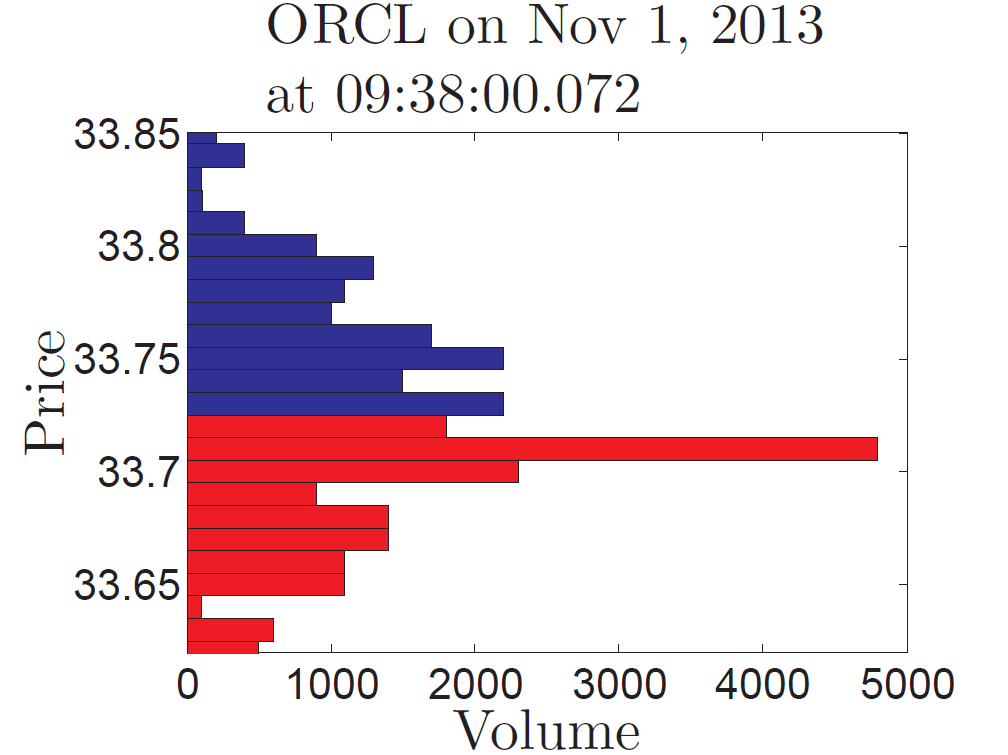
\includegraphics[scale=.65]{LOBex.PNG}
    \caption{Snapshot of the LOB for the ticker ORCL (Oracle) after the 10 000th event during that day. Blue bars indicates sell limit orders, whilst red bars are buy limit orders.}
    \label{fig:2}
\end{figure}

More formally according to \textcite{bouchaud2018trades} we can see an order as a tuple consisting of sign/direction ($\varepsilon_{x}$), price ($p_{x}$), volume ($v_{x}$) and submission time ($t_{x}$):
\begin{equation}
    \label{eq:0}
    x = (\varepsilon_{x}, p_{x}, v_{x}, t_{x})
\end{equation} Where $\varepsilon = \pm 1$ indicates if it is a buy or sell order and $v_{x} > 0$.. An example of a limit order book is shown above in \autoref{fig:2}. Market orders are other types of orders found on LOB markets, which are usually considered to be more aggressive. This as they seek to execute a trade immediately \parencite{cartea2015algorithmic}. For instance if a market order is placed and the quantity is larger then quantity available in the book. The order is \textit{re-routed} or sad to 'walk the book' until the order is filled \parencite{hasbrouck2007empirical,cartea2015algorithmic}.
\newline
\newline
When submitting an order $x$, the trader must chose the size $v_x$ and price $p_{x}$ according to a relevant \textit{lot size} and \textit{tick size} of the LOB \parencite{bouchaud2018trades}. The lot size $v_0$ is the smallest amount of the asset that can be trades. Hence the size of each order is a multiple of the lot size $v_{x} \in \{kv_{0} | k = 1,2,...\}$. The tick size $\vartheta$ is the smallest permissible price interval between different order within a given LOB \parencite{bouchaud2018trades}. The values of $v_{0}$ and $\vartheta$ differs a lot between exchanges. However expensive stocks are often traded with $v_0 = 1$ whilst cheaper stocks are traded with $v_{0} \gg 1$. In equity markets $\vartheta$ is often 0.01\% of the stocks's mid-price \parencite{bouchaud2018trades}. 
\newline
\newline
Both the tick size and lot size affect trading. As the lot size dictates the smallest permissible order size. Whilst the tick size $\vartheta$ dictates how much more expensive it is for a trader to gain the priority. Of choosing a higher or lower price to a buy or sell order \parencite{bouchaud2018trades}. Sometimes it is also useful to consider the \textit{relative tick size} $\vartheta_r$, which is equal to the $\vartheta$ divided by the mid-price for a given asset \parencite{bouchaud2018trades}. To make things more complicated modern markets has a lot of different order types. Such as \textit{hidden, reserved, iceburg} and \textit{Fill-or-Kill} orders just to mention a few. Where \parencite{foucault2013market, cartea2015algorithmic, hasbrouck2007empirical} gives a good overview of these. There also exist \textit{hybrid markets} which are traditional quote-driven markets as Nasdaq and London Stock Exchange (LSE) \parencite{foucault2013market}.

\subsection{Price Formation \& Discovery}

The mechanism of price formation is at the very heart of economics.  Which is also important to understand 'stylized facts' in financial price series as \textit{heavy tails} and \textit{volatility clustering}  \parencite{abergel2012market}. \text{Price discovery} is the speed and accuracy with which transactions prices incorporate information available to market participants \parencite{foucault2013market}. In fact market makers, professional traders who stand willing to buy or sell securities. Is a logical starting point for how prices are actually determined in the market \parencite{madhavan2000market}. Another key is also the role of information and who has it, that will be covered more in section .. \parencite{cartea2015algorithmic}.


\begin{figure}[H]
    \centering
    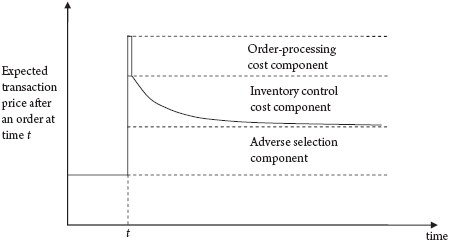
\includegraphics[scale=1]{bidask.png}
    \caption{Three components of bid-ask spread in short-term and lon-term response to a market buy order. Source: \textcite{foucault2013market}}
    \label{fig:3}
\end{figure}


\subsubsection*{Bid-Ask Spread}

The bid-ask spread is usually decomposed into three components: \textit{adverse selection, order-processing costs} and \textit{inventory holding costs} \parencite{foucault2013market}. Order processing costs, consists of the setup price and operating costs of trading. Inventory costs is cost associated with carrying inventory. Adverse selection costs are costs that arise because some traders are more informed then others. When trading with these \textit{informed traders}, market makers will on average lose money \parencite{darley2007nasdaq}. Therefore a fraction of the bid-ask spread can be seen as a compensation for having to trade against informed traders \parencite{darley2007nasdaq}.In \autoref{fig:3} above these are illustrated on a short-term and long-term perspective.
\newline
\newline
Market makers quote two prices the bid price and the ask price where the difference between these is the market makers \textit{spread} \parencite{madhavan2000market}. By doing this market makers are also providing \textit{liquidity} to the market. Spreads measure the execution cost of small transaction, by measuring how close the price of a trade is to the \textit{market price}. Where the market price is the \textit{equilibrium price} i.e. the price where demand equals supply \parencite{cartea2015algorithmic}. One approach is by using the \textit{midprice} in \autoref{eq:1}:

\begin{equation}
    \label{eq:1}
    S_{t} = \frac{1}{2}(a_t + b_t)
\end{equation}
Which is the simple average of the bid ($b_t$) and ask($a_t$) price.
However the most common spread measures are the \textit{quoted} and the \textit{effective} \parencite{cartea2015algorithmic, foucault2013market} spread both shown in \autoref{eq:2} and \autoref{eq:3}

\begin{equation}
    \label{eq:2}
    QS_t = a_t - b_t
\end{equation}

\begin{equation}
    \label{eq:3}
    ES_t = a_t - S_t \text{ or } ES_t = S_t - b_t
\end{equation}
The quoted spread represents the potential cost of immediacy at any point in time as well as the distance from the market price \parencite{cartea2015algorithmic}. As mentioned in \textcite{foucault2013market} the quoted spread is also a good measure of trading costs for small orders used for measuring liquidity. If we normalize \autoref{eq:2} with the mid price we get the \textit{relative quoted spread} 

\begin{equation*}
    RQS_t = \frac{a_t - b_t}{S_t}.
\end{equation*}
Another related measure is the so called \textit{relative weighted average bid-ask spread} (RTWAS):

\begin{equation}
\label{eq:4}
    RTWAS_{t} = \frac{\bar{a}(q) - \bar{b}(q)}{S_t}
\end{equation}
Where $\bar{a}(q)$ and $\bar{b}(q)$ is the average execution price for buy and sell market orders of size $q$ \parencite{foucault2013market}. On the other hand the effective spread or half-spread measures the realized difference between the price paid and the midprice. Which can also be negative indicating that one is buying at a price below or selling above the 'market price' \parencite{cartea2015algorithmic}. ES and QS differ in the fact that ES can only be measured when there is a trade while QS are always observable \parencite{cartea2015algorithmic}. Some stylized facts know about the bid-ask spread are \parencite{hasbrouck2007empirical, madhavan2002market, bouchaud2018trades}:
\begin{itemize}
    \item The trade prices series is a martingale \& the order flow is not symmetric
    \item The spread declines over time \& the bid-ask spread are lower in high volume securities and wider for more riskier securities.
    \item For large-tick stock, the spread is almost equal to on tick. Small-tick stocks have a broader distribution of spreads.
    \item There is a price impact of trades i.e. on average the arrival of a buy trade causes prices to rise ($S_t$ increases). Whilst the arrival of sell trades causes prices to fall ($S_t$ decreases).
\end{itemize}

\subsubsection*{Liquidity}
If the structure of a securities market is compared to a car design, measuring liquidity is like assessing the car's driving performance \parencite{foucault2013market}.Liquidity impounds the usual economic concept of \textit{elasticity}. In a liquid market, a small shift in supply and demand doesn't result in large price changes \parencite{hasbrouck2007empirical}. However liquidity is also concerned with trading costs. Market makers are seen as liquidity providers (sell-side) whilst liquidity demanders are the customers (buy-side) \parencite{hasbrouck2007empirical}. A key dimension of liquidity is \textit{immediacy}. This is the ability of a investor to buy or sell an asset without having to wait to find a counterpart. With an offsetting position to sell or buy \parencite{cartea2015algorithmic}. In fact the bid-ask spread is a common measure of how liquid a market is \parencite{foucault2013market}.

\subsubsection*{Other measures of implicit trading costs}
A popular benchmark in trading costs analysis is the \textit{volume-weighed average price} (VWAP). For all transaction in the stock during a interval ($T$), often a trading day \parencite{foucault2013market}:

\begin{equation}
    \label{eq:5}
    VWAP = \sum_{t\in T}{w_t p_t}
\end{equation}
Where $w_t = \frac{|q_t|}{\sum_{t\in T}{|q_t|}}$ and $p_t$ and $q_t$ is the price and size of the $t^{th}$ trade. Investors evaluate their broker's performance in getting a good price for their order, by comparing their own price with the day's VWAP \parencite{foucault2013market}. Another concern for participants that wish to execute large orders, is that they will have an adverse \textit{price impact}. That is, increasing the price when buying aggressively and lowering it when selling \parencite{cartea2015algorithmic, bouchaud2018trades}. A normal way of measuring this, is running a regression on the change of the midprice of the form below:

\begin{equation}
    \label{eq:6}
    \Delta S_n = \lambda q_n + \varepsilon_n
\end{equation}
Where $\Delta S_n = S_{n\tau}-S_{(n-1)\tau}$ for a time interval $[(n-1)\tau, n\tau]$ \parencite{cartea2015algorithmic}. Using \autoref{eq:6} we can then estimate $\lambda$. Where the parameter $\lambda$ also called \textit{Kyle's lambda} \parencite{bouchaud2018trades} is capturing the market's price reaction i.e. its price impact. On the other hand $q_n$ is the order imbalance or net order flow \footnote{difference between of buy and sell orders during an interval} and  $\varepsilon_n$ the error term assumed to be normally distributed \parencite{cartea2015algorithmic, foucault2013market}. In terms of measuring liquidity a lower $\lambda$ indicates that the market is more liquid. Due to greater competition, lower risk tolerance or lower volatility \parencite{cartea2015algorithmic}. Thus meaning that a lower $\lambda$ means that prices are less sensitive to order imbalance \parencite{foucault2013market}.  A larger $\lambda$ indicates that the given volume impacts the prices, and trading is thus more expensive \parencite{bouchaud2018trades}.

\subsection{Inventory-based models}
A large (positive) inventory causes the dealer or market maker to face a higher cost for observing more inventory. Which lowers both bid and ask prices by the same amount \parencite{o1995market}. Vice versa holds for negative inventory. 

\subsubsection*{Ho \& Stoll Model}
In \textcite{ho1981optimal} a model that handles the risk the market maker faces when providing his service is presented. In the model the following assumptions are made:

\begin{itemize}
    \item Transactions follow a stationary continuous time stochastic jump process i.e. a Poisson process. 
    
    \item The arrival rate of buy orders ($\lambda_a$) and sell orders ($\lambda_b$) will depend on the dealer's ask and bid prices.
    
    \item The dealer face uncertainty over the future value of his portfolio $X$
\end{itemize}
In the the absence of any transactions the portfolio growth $dX$ is given below:

\begin{equation}
    \label{eq:8}
    dX = r_{x}Xdt + XdZ_x
\end{equation}
Where $r_x$ is the mean return, $dZ_x$ is the Wiener process with mean zero variance $\sigma^{2}_X$. The dealers wealth is divided into three components: \textit{cash, inventory} and \textit{base wealth}. The value of the cash account ($F$) is:

\begin{equation}
    \label{eq:9}
    dF = rFdt- (p-b)dq_b + (p+a)dq_a
\end{equation}
Which changes with buys and sells of securities earning the risk-free rate $r$. The dealers inventory ($I$) is given by:

\begin{equation}
    \label{eq:10}
    dI = r_{I}Idt+pdq_{b} - pdq_{a} + IdZ_{I}
\end{equation}
The inventory consists of shares in the stock tha market maker makes.
Finally base wealth ($Y$) is given by:

\begin{equation}
    \label{eq:11}
    dY = r_{Y}Ydt+YdZ_{Y} 
\end{equation}
The objective of the dealer is now to maximize the expected utility of his total wealth $E[U(W_T)]$ at time horizon $T$, where 

\begin{equation}
    \label{eq:12}
    W_{T} = F_{T} + I_{T} + Y_{T}
\end{equation}
\autoref{eq:12} is what is termed \textit{the dealers pricing problem}. This is in fact an optimization problem where we want to maximize the value function $J(\cdot)$ using dynamic programming. We have thus the optimization below in \autoref{eq:13a}

\begin{equation}
    \label{eq:13a}
    J(t,F,I,Y) = \underset{a,b}{\max}[E[U(W_T)] | t,F,I,Y]
\end{equation}
where $U$ is the utility function, $a$ and $b$ are the ask and bid adjustments and $t, F, I,Y$ are the states variables time, cash, inventory and base wealth \parencite{o1995market}. The function $J(\cdot)$ gives the level of utility given that the dealer's decisions are made optimally \parencite{o1995market}. As there are no intermediate consumption before time $T$ in this model. The recurrence relation found by using the principle of optimality is:

\begin{equation}
    \label{eq:13bc}
    \underset{a,b}{\max}dJ(t,F,I,Y)=0 \text{ and } 
    J(T,F,I,Y)=U(W_T)
\end{equation}
Solving \autoref{eq:13bc} finds a solution to the dealer's problem, where we have to find the ask and bid prices for each state. To solve \autoref{eq:13bc} one requires to use stochastic calculus. By writing out the partial differential equations that \autoref{eq:13bc} implies and apply Ito's Lemma:

\begin{align*}
    \label{eq:13d}
    \underset{a,b}{max}(dJ/dt) = & J_t + LJ \\
    & + max\{\lambda_a[J(F+pQ+aQ, I-pQ,Y) - J(F,I,Y)] \\
    & + \lambda_b [J(F-pQ+bQ, I+pQ,Y) - J(F,I,Y)] \} = 0 \numberthis
\end{align*}
where $J_t$ is the time derivative and $L$ is the operator defined as

\begin{equation}
    LJ = J_{F}rF + J_{I}r_{I}I+J_{Y}r_{y}Y+\frac{1}{2}J_{II}\sigma^{2}_{I}I^{2}+ \frac{1}{2}J_{YY}\sigma^{2}_{Y}Y^{2} + J_{IY}\sigma_{IY}IY
\end{equation}
$J_t + LJ$ is the total time derivative of derived utility when there are no transactions. \autoref{eq:13d} determines the solution, but is hard to solve explicitly. \textcite{ho1981optimal} do not solve the general problem but introduces some transformations and simplifications in order to solve it. Firstly by looking at the problem only at the endpoint ($\tau$) is equal to zero. Secondly \parencite{o1995market} .. and define two new operators sell ($S$) and buy ($B$) operators:
\begin{align}
    \label{eq:13e}
    SJ = & S[J(F,I,Y)] = J(F+Q,I-Q, Y) \\
    BJ = & B[J(F,I,Y)] = J(F-Q, I+Q, Y)
\end{align}

By using the new operators the problem in \autoref{eq:13d} can be rewritten as

Which gives the bid and ask prices
\begin{align}
\label{eq:13f}
    b^{*} = & \alpha/2\beta + (J-BJ)/2BJ_{F}Q \\
    a^{*} = & \alpha/2\beta + (J-SJ)/2SJ_{F}Q \label{eq:13g}
\end{align}
From \autoref{eq:13f} and \autoref{eq:13g} we get the bid-ask spread as
\begin{equation}
    \label{eq:13h}
    s = \alpha / \beta + (J-SJ)/2SJ_{F}Q + (J-BJ)/2BJ_{F}Q
\end{equation}
\textcite{ho1981optimal} demonstrates three important properties of the dealer's optimal pricing behavior:

\begin{enumerate}
    \item The spreads depends on the time horizon of the dealer
    \item The spread can be decomposed into a risk neutral spread plus an adjustment for uncertainty
    \item The spread is independent of inventory level.
\end{enumerate}

\subsection{Information-based models}

\subsubsection*{Glosten-Milgrom Model}
In the Glosten-Milgrom one tries to capture the features of how adverse selection affects the bid ask spread \parencite{darley2007nasdaq}. One assumes the following in the model:
\begin{itemize}
    \item A market with trading in a single asset
    \item All market participants are risk-neutral and act competitively
    \item The market is \textit{frictionless} i.e. there are no transaction costs, taxes or holding costs.
    \item The value of the asset is a random variable whose probability law is know to the market makers.
\end{itemize}
Informed traders have information about the realization of a assets \textit{true value}, $V$. The distribution of $V$ is assumed to be binomial. With the probability $\theta$ and $1- \theta$ if the value of the asset is higher or lower $\overline{V}, \underline{V}$  then the true value \parencite{darley2007nasdaq}. Uniformed traders only have information about the triple $(\theta, \underline{V}, \overline{V})$ and we have two fraction of these. The ones that wants to buy $\gamma^{B}$, and the ones that want to sell $\gamma^{S}$ \parencite{darley2007nasdaq}. The fraction of informed traders is instead denoted $\mu$. The market maker sets bid ($E[V|\text{Sell}]$) and ask prices ($E[V|\text{Buy}]$) by conditional expectations of the true value given a sell or buy order. By definition \parencite{darley2007nasdaq} 
\begin{equation}
    \label{eq:7}
    E[V|\text{Sell}] = \underline{V}P[V=\underline{V}|\text{Sell}] + \overline{V}P[V=\overline{V}|\text{Sell}]
\end{equation}
And by using Bayes' rule the probabilities  can be obtained, for instance $P[V=\overline{V}|\text{Sell}] = \frac{\theta(1-\mu)\gamma^{S}}{(1-\mu)\gamma^{S} + (1-\theta)\mu}$.
Note that the Glosten-Milgrom model has no actual auction mechanism. Which makes the model inadequate for studying the effect of microstructure on non-equilibrium market behavior \parencite{darley2007nasdaq}.

\subsubsection*{Das Model}

%\subsection{Empirical metrics}

\newpage

\section{Artificial Financial Markets}
In agent-based modelling (ABM), appropriate parts of the complex system are modeled as autonomous decision-making entities called \textit{agents} \parencite{darley2007nasdaq}. In ABM market investors or traders are modelled as agents trading together via an orderbook \parencite{lussange2018bright}. However the decision of what type of agents to use is paramount. Where a wide range of of different types of agents from \textit{zero-intelligence agents} to \textit{reinforcement learning agents} \parencite{martinez2009evolutionary}. Broadly speaking there is a price disagreement between the agents, where often pricing is done randomly also called \textit{noise traders}. Or via some real world strategy \parencite{lussange2018bright}. According to \textcite{martinez2009evolutionary} some important design issues to think about are:

\begin{itemize}
    \item \textit{Decision making} i.e. is it rule based, or based on something else.
    \item \textit{Objective function} i.e. explicit, implicit or utility or profit maximization.
    \item \textit{Heterogeneity} i.e. types of agents, parameters, information basis and learning.
    \item \textit{Learning} i.e. zero intelligence or more complex.
\end{itemize}
Validation is an important issue in agent-based modelling, where simulated markets should be able to replicate realistic quantitative features of the real market, with reasonable calibration \parencite{martinez2009evolutionary}. In order to validate multiple parameters need to be user defined. However to overcome this, using a benchmark in which the behaviour of the market is well defined is on way. Another way according to \textcite{martinez2009evolutionary} is to use parameters in the simulated market derived from experimental or real markets. 
\newline
\newline
It is also common to test whether the prices created via the interaction of the agents exhibit certain \textit{stylized facts}. That real world markets do \parencite{brandouy2011design}. With stylized facts we mean a set of properties that is common across many instruments, markets and times. That has been observed by independent studies \parencite{cont2001empirical}. Where some of the know stylized facts important for this study are:

\begin{itemize}
    \item \textit{Absence of autocorrelations} i.e. linear autocorrelations are often insignificant. 
    \item \textit{Non Gaussian returns \& Heavy tails} i.e.the unconditional distribution of returns seems to display a power-law or Pareto-like tail.
    \item \textit{Volatility clustering}. 
\end{itemize}
For more information see for instance \textcite{cont2001empirical}.

%mention what it is, some strategies, and how it effect modern markets
\section{Algorithmic and High-Frequency Trading}
Algorithmic trading consists in using computer programs to implement investment and trading strategies \parencite{abergel2012market}. Conversely, High frequency trading (HFT)is a term used to describe a large diverse set of activities and behaviors \parencite{o2015high}. Where some of the main characteristics for high frequency traders are: (i) use of \textit{high-speed} and sophisticated programs for \textit{generating, executing} and \textit{routing} orders, (ii) use of \textit{co-location} to minimize \textit{latency}, (iii) very short time frames for their positions, (iv) submission of numerous orders that are cancelled shortly and (v) ending the day with almost flat positions. 
\newline
\newline
A distinction can be made between algorithmic trading and HFT in their order frequency. Where HFT can enter more than thousands of orders per second, while algorithmic trading enters a few orders per minute \parencite{abergel2012market}.

\subsection{Different types of strategies}

\subsubsection*{Optimal Executions}

\subsubsection*{Targeting volume}

\subsubsection*{Market Making}

\subsubsection*{Pairs Trading \& Statistical Arbitrage}
\textit{Pairs trading} is a portfolio that consists of a linear combination of two assets that are traded \parencite{cartea2015algorithmic}. At the heart of the strategy is how the two assets co-move. Pairs trading algorithms profit from betting on the fact that spread deviations tend to return to historical or predictable levels \parencite{cartea2015algorithmic}. Which makes it fall under the class of strategies called \textit{statistical arbitrage}.

\subsection{Cost and benefits}

\section{Reinforcement Learning}
Reinforcement learning (RL) is learning what to do i.e. map situations to actions, in order to maximize a numerical reward function \parencite{sutton1998reinforcement}. Which is quite different from other machine learning methods based on \textit{supervised} or \textit{unsupervised} learning, where one in fact have the true labels or not.
\subsection{The Main Concepts}
\begin{figure}[H]
    \centering
    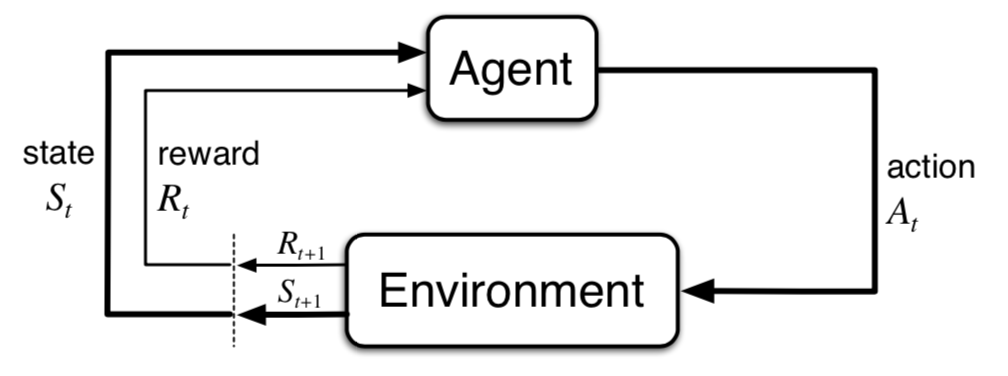
\includegraphics[scale=1]{basicRL.png}
    \caption{Basic overview of the reinforcement learning setting with an agent interacting via actions ($A_t$) with it's environment moving through states ($S_t$). Thus gaining different rewards ($R_t$). Source: \textcite{sutton1998reinforcement} }
    \label{fig:4}
\end{figure}

Reinforcement learning (RL) is about an agent interacting with the environment. By learning an optimal policy, by trial and error. For sequential decision making \parencite{li2017deep}. \autoref{fig:4} above illustrates a simple agent interacting with its environment. A RL agent interacts with its environment over time. At each time step $t$ the agent receives  a \textit{state} $S_t$ in a state space $\mathcal{S}$ and makes an \textit{action} $A_t$ from an action space $\mathcal{A}$ \parencite{li2017deep}. As a consequence of its action, the agent receives \textit{reward} $R_t$ which is a scalar value. The agent's goal is to maximize the total amount of cumulative reward it receives. This is know as the \textit{reward hypothesis} \parencite{sutton1998reinforcement}. The agent's behavior is modelled by the \textit{policy} $\pi(s|a)$. A policy is a mapping from a state to an action, that is the probability of selecting action $A_t=a$ if state $S_t = s$. 
\newline
\newline
This also includes transitioning to the next state $S_{t+1}$ according to the environments dynamics or \textit{model} for a \textit{reward function} $\mathcal{R}(s,a)$ and \textit{state transition probability}
\subsubsection*{Markov Decision Process}
$\mathcal{P}(S_{t+1} |S_t, A_t)$ \parencite{li2017deep}. More formally the RL problem is formulated as an \textit{Markov Decision Process} (MPD) \parencite{sutton1998reinforcement, li2017deep}. A MDP is a tuple $(\mathcal{S, A, P, R}, \gamma)$ \parencite{li2017deep}:
\begin{itemize}
    \item $\mathcal{S}$ is a finite set of states
    \item $\mathcal{A}$ is a finite set of actions
    \item $\mathcal{P}$ is a transition probability matrix, 
    \begin{equation} 
        \label{eq:12a}
        \mathcal{P}^{a}_{ss'} = P[S_{t+1} = s' | S_t =s, A_t = a]
    \end{equation}
    \item $\mathcal{R}$ is a reward function, 
    \begin{equation}
        \label{eq:12b}
        \mathcal{R}^{a}_{s} = E[R_{t+1} | S_t =s, A_t=a]
    \end{equation}
    \item $\gamma \in [0,1]$ is a \textit{discount factor} 
\end{itemize}
In general, we seek to maximize the \textit{expected return}. Where the return, denoted $G_t$ is total discounted reward from time step $t$:

\begin{equation}
    \label{eq:13}
    G_t = R_{t+1} + \gamma R_{t+2} + ... = \sum_{k=0}^{\infty}{\gamma^{k}R_{t+k+1}}
\end{equation}
The discount factor or discount rate in \autoref{eq:13} determines the present value of future rewards, $k$ steps in the future. Note that a $\gamma$ close to 0 leads to \textit{myopic} behavior i.e. the agent only cares about immediate rewards. Whilst if $\gamma$ is close to 1, the agent's is a bit more \textit{far-sighted}. When the agent-environment interaction breaks naturally into sub-sequences which is called \textit{episodes}
\autoref{eq:13} makes sense.  Another key concept underlying RL is the \textit{Markov property} i.e. only the current state affects the next state \parencite{arulkumaran2017brief}. More formally this means:

\begin{equation}
    \label{eq:13b}
    P[S_{t+1} | S_t] = P[S_{t+1} | S_1, ..., S_t]
\end{equation}
\autoref{eq:13b} states that the future is conditionally independent of the past given the present state. According to \textcite{arulkumaran2017brief} this assumption is somewhat unrealistic. As it requires the states to be fully observable. A generalization of a MDPs are partially observable MDPS (POMDPS). In which the agent receives an observation $O_t \in \mathcal{O}$. Where the distribution of the observation is $P(O_{t+1} | S_{t+1} | A_t)$\parencite{arulkumaran2017brief}. Which is dependent on the current state and the previous action.

\subsubsection*{Value Functions}

Almost all RL algorithms involve estimating \textit{value functions} i.e. functions of states or state-action pairs. These estimate how god it is for an agent to be in a certain state \parencite{sutton1998reinforcement, li2017deep}. The value of a state $s$ under a policy $\pi$ denoted $v_{\pi}(s)$. Is the expected return when starting in $s$ and following $\pi$. Below is the \textit{state-value function for policy $\pi$}:

\begin{equation}
    \label{eq:14}
    v_{\pi}(s) = E_{\pi}[G_t | S_t = s] = E_{\pi}\left[\sum_{k=0}^{\infty}{\gamma^{k}R_{t+k+1}} | S_t = s\right], \forall s \in \mathcal{S}.
\end{equation}
Note that the value of the terminal state is always zero \parencite{sutton1998reinforcement}. Similarly  we can define the the \textit{action-value function for policy $\pi$} \parencite{sutton1998reinforcement}. Which is the value of taking action $a$ in state $s$ under policy $\pi$, denoted $q_{\pi}(s,a)$. Is the expected return starting from $s$, taking the action $a$ and therefore following policy $\pi$:

\begin{equation}
    \label{eq:15}
    q_{\pi} = E_{\pi}[G_t | S_t =s, A_t = a] = E_{\pi} \left[\sum_{k=0}^{\infty}{\gamma^{k}R_{t+k+1}} | S_t=s, A_t=a \right]
\end{equation}
Both \autoref{eq:14} and \autoref{eq:15} can be estimated from experiences or by using \textit{Monte Carlo Methods} \parencite{sutton1998reinforcement}.

\subsubsection*{Bellman equations \& Optimality}
Both \autoref{eq:14} and \autoref{eq:15} satisfies recursive relationships. Which is commonly know as \textit{Bellman equations} \parencite{sutton1998reinforcement}:

\begin{equation}
    \label{eq:16}
    v_{\pi} = E[G_t | S_t = s] = E_{\pi}[R_{t+1} + \gamma G_{t+1} | S_t = s]
\end{equation}

\begin{equation}
    \label{eq:17}
    q_{\pi} = E_{\pi}[R_{t+1} + \gamma G_{t+1} | S_t = s,  A_t = a]
\end{equation}
As we can see in \autoref{eq:16} and \autoref{eq:17} the Bellman equations expresses a relationship between the value of the state and its successor states. However solving a RL task means that we want to find a policy that achieves a lot of reward over the long run. We are thus looking for \textit{optimal policies} ($\pi \geq \pi'$). We denote all optimal policies with $\pi_{*}$ whom share the same state-value and action value-value functions \parencite{sutton1998reinforcement}. We thus want to maximize the following:

\begin{equation}
    \label{eq:18}
    v_{*}(s) = \underset{\pi}{\text{max }} v_{\pi}(s)
\end{equation}

\begin{equation}
    \label{eq:19}
    q_{*}(s,a) = \underset{\pi}{\text{max }} q_{\pi}(s,a)
\end{equation}

Using \autoref{eq:18} and \autoref{eq:19} together with the Bellman equation in \autoref{eq:16} and \autoref{eq:17} we get the \textit{Bellman optimality equations}:

\begin{equation}
\label{eq:20}
\begin{aligned}
& & v_{*}(s) =  \underset{a}{\text{max }} 
E_{\pi_{*}}[R_{t+1} + \gamma v_{*}(S_{t+1}) | S_t =s, A_t = a] \\
& & = \underset{a}{\text{max }} 
\sum_{s', r}^{}{p(s', r | s,a)}[r + \gamma v_{*}(s')]
\end{aligned}
\end{equation}

\begin{equation}
\label{eq:21}
\begin{aligned}
& & q_{*}(s,a) = 
E[R_{t+1} + \gamma \underset{a'}{\text{max }}q_{*}(S_{t+1, a'}) | S_t =s, A_t = a] \\
& & =  \sum_{s', r}^{}{p(s', r | s,a)}[r + \gamma \underset{a'}{\text{max }}q_{*}(s',a')]
\end{aligned}
\end{equation}
For a finite MDP \autoref{eq:20} and \autoref{eq:21} has a unique solution independent of the policy \parencite{sutton1998reinforcement}. Nevertheless, in practice there is no closed form solution for these equations. Therefore one must resort to approximate and iterative methods. That uses \textit{dynamic programming} or Monte Carlo methods.

\subsection{Exploration versus Exploitation}
In reinforcement learning we have a trade-off between \textit{exploration} and \textit{exploitation}. Where exploration refers to taking actions, that come from the current best version of the learned policy. Exploration instead is concerned with taking more actions to obtain more training data \parencite{goodfellow2016deep}. Where the dilemma is that neither exploration nor exploitation can be pursued exclusively without failing at the task \parencite{sutton1998reinforcement}. There exist some strategies to balance the trade-off between exploration and exploitation. By employing a \textit{greedy} approach i.e. choose the action with the highest payoff \parencite{sutton1998reinforcement, szepesvari2009algorithms}.

\begin{equation}
    \label{eq:21a}
    A_t = \underset{a}{\operatorname{argmax}}Q_t(a)
\end{equation}
A simple modification of \autoref{eq:21a} is to fix $\varepsilon > 0$ and choose a random selected action. With probability $\varepsilon$ and go with the greedy choice else. This strategy is the $\varepsilon$-greedy one. Another approach is \textit{Boltzman exploration} \parencite{sutton1998reinforcement,szepesvari2009algorithms} which given the sample means of the actions at time $t$. The next action is drawn from the multinominal distribution of $\pi_t$, where 

\begin{equation}
    \label{eq:21b}
    P_t(a) = \frac{\exp{(q_{t}(a)/\tau)}}{ \sum_{i=1}^{n}{\exp{(q_{t}(i)/ \tau)}}} = \pi_t(a)
\end{equation}
Where $ \tau$ is a temperature parameter annealed over time.
Finally there also exist approaches based on the \textit{optimism in the face of uncertainty}. According to which where the learner should choose the action with the best upper confidence bound (UCB) \parencite{sutton1998reinforcement, szepesvari2009algorithms}

\begin{equation}
    \label{eq:21c}
    A_t = \underset{a}{\operatorname{argmax}} \left[Q_t(a) + c \sqrt{\frac{\ln{t}}{N_t(a)}} \right]
\end{equation}
Where $t$ is the time, $c$ controls the degree of exploration and $N_t(a)$ is the number of times that action $a$ has been selected \parencite{sutton1998reinforcement}.

\subsection{Algorithms \& Learning in RL}
One can characterize RL problems into two main classes: \textit{prediction} and \textit{control} where each is followed by different approaches as \textit{value iteration, policy iteration} and \textit{policy search} \parencite{szepesvari2009algorithms}. 
\newline
These different approaches uses different algorithms. Note that all these algorithms are implemented in both \parencite{plappert2016kerasrl, baselines} libraries used in the thesis. In general deep reinforcement learning is based on the algorithms below, but with deep neural networks. To approximate $V^{*}, Q^{*}$ and $A^{*}$ \parencite{arulkumaran2017brief}. 

%neeed this? maybe put in appendix..
\subsubsection*{Dynamic Programming \& Monte Carlo Methods}
In order to find optimal solutions for \autoref{eq:20} and \autoref{eq:21} we must resort to using approximate methods as dynamic programming. The key idea of dynamic programming is to use the value functions to organize and structure the search for good policies \parencite{sutton1998reinforcement, szepesvari2009algorithms}. Once a policy $\pi$ has been improved using $v_{\pi}$ to yield a better policy,  $\pi'$. We can then compute $v_{\pi}'$ and improve it again to yield policy $\pi^{''}$ \parencite{sutton1998reinforcement}. This is what \textit{policy iteration} is about and is described more in \autoref{alg1} found in \autoref{app:A}.
\newline
\newline
One drawback with \autoref{alg1} is that is quite computationally expensive as it involves policy evaluation over the state space \parencite{sutton1998reinforcement}. A remedy for this is \textit{value iteration}. Where the basic idea is to use early stopping i.e. one update of each state. Which is shown in \autoref{alg2} in \autoref{app:A}. Conversely \textit{Monte Carlo methods} (MCM) require only experience i.e. sample sequences of states, actions, and rewards. From actual or simulated interaction with the environment \parencite{sutton1998reinforcement}. MCM solves reinforcement learning problems based on averring sample returns. 


\subsubsection*{Q-Learning \& SARSA}
\textit{Temporal difference} (TD) learning can be seen as a combination of Monte Carlo methods and dynamic programming. That learn directly from raw experience without a model of the environment's experience \parencite{sutton1998reinforcement, arulkumaran2017brief}. The most simple TD method makes the following update:

\begin{equation}
    \label{eq:22}
    V(S_t) \leftarrow V(S_t) + \alpha \left[R_{t+1} + \gamma V(S_{t+1} - V(S_t) \right]
\end{equation}
This idea is applicable both to \textit{Q-Learning} and \textit{State-action-reward-state-action} (SARSA) which are both cases of TD learning. However Q-Learning is a \textit{off-policy} method whilst SARSA is an \textit{on-policy method} \parencite{sutton1998reinforcement, arulkumaran2017brief}. Now we are interested in learning an \textit{action-value} function which we estimate with $Q^{}$, instead of a state-value function. The update rule for SARSA is given below in \autoref{eq:23}:

\begin{equation}
    \label{eq:23}
    Q(S_t, A_t) \leftarrow Q(S_t, A_t) + \alpha \left[R_{t+1} + \gamma Q(S_{t+1}, A_{t+1}) - Q(S_t, A_t) \right]
\end{equation}
Q-learning instead estimates  $q_{*}$ \footnote{The optimal action-value function} with the learned action-value function $Q$ independent of the policy being followed \parencite{sutton1998reinforcement}. 
%\newpage
The main update rule for \textit{Q-learning} is given below in 

\begin{equation}
    \label{eq:24}
     Q(S_t, A_t) \leftarrow Q(S_t, A_t) + \alpha \left[R_{t+1} + \gamma \underset{a}{\operatorname{max}} Q(S_{t+1}, a) - Q(S_t, A_t) \right]
\end{equation}

\subsubsection*{Deep Q Networks (DQN}
In \textcite{mnih2015human} from Google DeepMind created Deep Q Learning (DQN). Which replaces the $Q$ function with a neural network called \textit{Q-network}. This method also keeps track of some observations in memory which is called \textit{experience replay} \parencite{mnih2015human}. The agents experience is stored $e_t = (s_t, a_t, r_t, s_{t+1})$ at each time step in a data set $D_t = \{e_1, ..., e_t\}$. Where on Q-learning updates the experience is drawn uniformly \parencite{mnih2015human}. They use a deep convolutional network to the approximate optimal action-value function $Q^{*}$. The Q-learning update at iteration $i$ uses the loss function in \autoref{eq:25} below:

\begin{equation}
    \label{eq:25}
    L_i(\theta_i) = \mathbb{E}_{(s,a,r,s') \sim U(D)} \left[\left(r+ \gamma \underset{a'}{\operatorname{max}}Q(s', a', \theta_{i}^{-})-Q(s,a;\theta_i)  \right)^2 \right]
\end{equation}
Where $\gamma$ is the discount factor, $\theta_i$ are the parameters of the Q-network. $\theta_{i}^{-}$ is the parameters of the target network \parencite{mnih2015human}.

%add full algorithm here

\subsubsection*{Policy Gradients \& Proximal Policy Optimization (PPO)}
Policy gradients methods work by  directly computing an estimate of the gradient of policy parameters in order to maximize the expected return. This by using stochastic gradient descent \parencite{bansal2017emergent}. 
Policy gradient methods work by computing an estimator of the policy gradient and plugin it in to a stochastic gradient ascent algorithm \parencite{schulman2017proximal}. The most common estimator is shown below in \autoref{eq:26}

\begin{equation}
    \label{eq:26}
    \hat{g} = \hat{\mathbb{E}}_{t}\left[\nabla_{\theta} \log{\pi_{\theta}(a_t|s_t)\hat{A}_{t}} \right]
\end{equation}
Where $\pi_{\theta}$ is a stochastic policy and $\hat{A}_{t}$ is an estimator of the advantages function at timestep $t$. The advantage function is shown below in \autoref{eq:27}:

\begin{equation}
    \label{eq:27}
    \hat{A}_{t} = -V(s_t) + r_t +\gamma r_{t+1} + ... \gamma^{T-t+1} r_{T-1} + \gamma^{T-t}V(s_T).
\end{equation}
In \textcite{schulman2017proximal} they propose a new family of policy gradient methods. That alternates between sampling data through interaction with the environment, and optimizing a "surrogate" objective function using stochastic gradient ascent.  The surrogate function that we want to optimize is given by \autoref{eq:28} below: 

\begin{equation}
    \label{eq:28}
    L_{t}^{CLIP + VF+ S}(\theta) = \hat{\mathbb{E}_{t}} = \left[L_{t}^{CLIP}(\theta) + c_1 L_{t}^{VF}(\theta) + c_2S[\pi_{\theta}(s_t)]\right]
\end{equation}
Where $c_1,c_2$ are coefficients, and S is an entropy bonus. $L_{t}^{CLIP}$ is the clipped surrogate objective and $L_{t}^{VF}$ is a squarred-error loss \parencite{schulman2017proximal}.
%add full algorithm here

\subsection{Competitive Self-Play}
Many real-world applications can be described as large-scale of games of imperfect information. A game is a domain of conflict for cooperation between several entities \parencite{heinrich2016deep}. Where the optimal solutions for these types of situations would be Nash equilibrium. That is an strategy from which no agent would choose to deviate \parencite{heinrich2016deep}. This is where self-play comes in. In short self-play is the activity of imagining or simulating the play of a game against oneself \parencite{heinrich2017reinforcement}. This concept is also based on the idea of \textit{fictitious play}.  Where fictitious players choose best responses to their opponents' average behaviour \parencite{heinrich2016deep}. 
\newline
\newline
\textcite{tampuu2017multiagent} also mentioned that self-play is any type of play against an \textit{adaptive agent}. Typically agents are first trained in a supervised manor, with self-play as a second phase of training. In \textit{Fictious Self-Play} (FSP) on the other hand the agents generate datasets of their experience in self-play \parencite{heinrich2016deep}.  Each agent stores transition tuples $(s_t, a_t, r_{t+1}, s_{t+1})$ in a memory $\mathcal{M}_{RL}$ for reinforcement learning (confer experience replay). Experience of the agent's own behaviour $(s_t, a_t)$ is stored in a separate memory for supervised learning $\mathcal{M}_{SL}$ \parencite{heinrich2016deep}.
\newline
\newline
\textcite{bansal2017emergent} mentioned that in a competitive-multi agent environment trained with self-play. Far more complex behaviours then the environment itself can emerge. In general training an agent to perform a highly complicated task requires a complicated environment, but there exists environments where behaviour of the agent is far more complex. Then the environment itself \parencite{bansal2017emergent}. These types of environments have two interesting properties:

\begin{enumerate}
    \item Very simple competitive multi-agent environments can produce extremely complex behavior
    \item When training with self-play the environment provides the agents with  a perfect curriculum.
\end{enumerate}

%mention where it has been succesfully used and show the need of the application that we want to use here for the thesis
%\subsection{RL in Market Microstructure}

\newpage

\subsection{Issues with deep RL}


%necessary?
%\section{Tree Search}

%\subsection{MinMax}

%\subsection{Monte Carlo Tree Search (MCTS)}

%own chapter?
\chapter{Related Work}
In this chapter previous related work is presented. To give a view over what has been done previously as well as current state of the art. Also the difference between this work and previous work is discussed. The chapter is divided into the following sections: \textit{Agent Financial Markets, Market Microstructure} and \textit{Reinforcement Learning in Finance}.

\section{Agent based Financial Markets}
The field of finance and economics have used various approaches to model financial markets dynamics. Among these three main groups of approaches can be distinguished: \textit{statistical models}, \textit{Dynamic Stochastic General Equilibrium (DSGE)} and \textit{Agent-Based Models (ABM)} \parencite{lussange2018bright}. Agent-based financial markets of different characteristics have been developed for some time. A early model is given in \parencite{raberto2001agent} where they in their 'Geona market' have agents adopting strategies as chartist, fundamentalist or random. A drawback with the model is that it doesn't manage to correctly represent the price behavior in the market \parencite{raberto2001agent}. In this thesis we aim to do so, by using reinforcement learning instead. 
\newline
\newline
Good overviews of agent based modelling in a financial setting, is given in \parencite{martinez2009evolutionary, boer2008agent, lebaron2006agent}. Where a more recent overview of agent based modelling in finance and economics is presented in \parencite{lussange2018bright}. In \textcite{martinez2009evolutionary} they introduce CHASM which is a software platform that allows user to experiment with different market scenarios. This market is composed of technical, fundamental and noise traders. 
\newpage
Where genetic programming seems to be the core learning process employed and decision trees. A difference between the study by \textcite{martinez2009evolutionary} and this thesis, is that the environment used will be more complex. With a matching engine and different algorithmic trading strategies as market making and HFT trading. To successfully study market microstructure phenomena. We will also use reinforcement learning for learning used by the agents in the complex environment. Generally speaking there are two major approaches to agent-based financial market simulations, where the first one focuses on specific market structure. Whilst the second approach is more focused on generating a flexible environment with flexible settings for the agents employed \parencite{brandouy2011design}. This thesis will focus more on the second approach in order to see what type of behaviour the agents exhibit exposed to different market conditions. 
\newline
\newline
In \textcite{brandouy2011design} they design a artificial stock market called ATOM based on the Euronext-NYSE Stock exchange, with the possibility to add ''human agents''. They have for instance a limit order-book as the thesis aim to use, but it is unclear whether they employ a functional matching engine. Which this study will use, by using the parity engine \footnote{\url{http://paritytrading.com/}}. They also use different types of agents for instance \textit{zero intelligence traders, technical traders, evolutionary agents, risk averse agents} and \textit{mean-variance agents}. 
\newline
\newline
Nevertheless, none of these are based on reinforcement learning or competitive self-play as will be used in this thesis. One of the main benefits with using agent based modelling is that they demonstrate the ability to produce realistic system dynamics, which are comparable to those observed empirically \parencite{platt2016problem}. In their study the calibrate their agents by using heuristic optimization , Nelder-Mead simplex algorithm and a genetic algorithm. They use a simpler form of matching engine, not as elaborated as the parity engine. They also only use a low-frequency trader and high-frequency trader. Where this thesis may use one or several different types of traders

\section{Market Microstructure}
Market microstructure studies the process by which investors' latent demands are ultimately translated into prices and volumes \parencite{madhavan2000market}. It is of importance for this thesis to understand market microstructure both theoretically and empirical. In order to replicate and even find new interesting behaviour of the agents, employed in this kind of environment. In \textcite{haferkorn2017high, agarwal2012high} the effect of HFT trading and fragmentation is discussed. Which is of interest for market micro-structure. This as fragmentation leads to more competition on the markets. That might be demonstrated by the agents. Some common references that have been and are still used in the state of the art market microstructure research is \parencite{o1995market,hasbrouck2007empirical, madhavan2000market, madhavan2002market}. There both \textit{inventory-based} and \textit{information based} models are discussed. In this thesis both an inventory-based and information based model will be used as a benchmark, for the learning agents. 
\newline
\newline
A common inventory-based model, that uses dynamic programming to find the optimal dealer price in a one-dealer market. Is given in \textcite{ho1981optimal}. A problem with the model in \parencite{ho1981optimal} is that here is no closed form solution, thus approximations is used to get arbitrarily close to the solution. By using reinforcement learning we hope to be able to replicate the behaviour of the agents shown in the previous paper. However, also extending it, and see how the agents perform and behave in a more complex market. With several dealers for instance. The information based models on the other hand tries to incorporate the element that some traders are more informed than others. Which is called \textit{asymmetric information} or \textit{adverse selection} in the market microstructure literature \parencite{o1995market, hasbrouck2007empirical}. 
\newline
\newline
A recent model for this is the one presented in \parencite{das2003intelligent, das2005learning}. Which is an extension of the model presented in \textcite{glosten1985bid}. The Glosten and Milgrom model derives the market makers price by setting equations under asymmetric information. To be such that the bid/ask quotes are the expectations conditioned on if the order is a buy or sell order. In \textcite{das2005learning} on the other hand they employ a non-parametric density estimate of the true value or fundamental value of the stock. This by using Bayesian Learning. 

\newpage
We will be training our agents on an environment similar to the one described in \parencite{das2005learning} but with reinforcement learning instead. We hope to see the same market dynamics as they did in their study. To further validate the agents learning of trading dynamics. Before using them on the more complex model with the matching engine. Finally in \textcite{o2015high} they mentioned that in a high-frequency world. Older empirical models may no longer be appropriate. Where this thesis aims to provide a step in a new direction for this type of research.

\section{Reinforcement Learning in Finance}

Reinforcement learning or \textit{neuro-dynamic programming} as it also have been called in the literature. Have been used previously in a financial setting. Where some of the earlier applications have been in trading. In \textcite{moody1999reinforcement} the author's explore the opportunity of using reinforcement learning for trading. Using Recurrent Reinforcement Learning (RRL) and Q-learning and looking at the S\& P 500 index. Not that much focus is on trading dynamics. Which will be the main focus of  this thesis, on a completely different market. In \parencite{dempster2006automated, du2016algorithm, wang2016reinforcement, casqueiro2006neuro, bertoluzzo2012testing} they discuss the usages of different types of reinforcement learning algorithms for trading. Where trading is done in for example foreign exchange or the energy market. None of these use a matching engine, or a more complex environment with several HFT/market maker agents. Or with the possibility of completely changing the market conditions. Which this thesis aims to do. 
\newline
\newline
In \textcite{kearns2013machine} they give a good overview of reinforcement learning used in market microstructure and high-frequency trading. With use-cases in optimized trade execution, prediction of price movements and optimized execution in dark pools. Nevertheless none of these studies are using competitive self-play in their learning. In \parencite{nevmyvaka2006reinforcement, hendricks2014reinforcement}  optimized trade execution is studied with the help of reinforcement learning. Which is of importance in market microstructure and might be examined in this thesis. However for this thesis one of the main objectives is to understand and successfully replicate know behaviour of traders in a dynamic market. Where some studies concerned with understanding the behaviour of traders are presented in \parencite{yang2014algorithmic, yang2012behavior}. 
\newline
\newline
Where they use \textit{inverse reinforcement learning} on trading decisions. The idea is to find the reward function given the observations of optimal trading behaviour and then use it for trader identification. 
Although interesting this thesis is not interested in capturing key characteristic of already optimal HFT strategies. Instead we want to see what optimal or not optimal behaviour the agents will use, and how they will react to changed market conditions. Therefore reinforcement learning is used instead. Another common application of reinforcement learning is also in market making see for instance \parencite{jumadinova2010comparison,chan2001electronic, fernandez2015high, sherstov2004three}. Market making strategies will be implemented in this thesis along with other algorithmic trading strategies. To make the market more plausible. 
\newline
\newline
In \textcite{cartea2015algorithmic} some common algorithmic trading strategies are presented, focusing on stochastic optimal control.
A previous study has been done at NASDAQ investigating the effects of tick size changes \textcite{darley2007nasdaq}. Where the strategies employed where a simpler form of reinforcement learning, together with dynamic programming approaches. This study is of-course used as an inspiration, but the thesis will be different in that it incorporates a more realistic market. With the matching engine, and several different types of agents. When modelling stock agents some previous studies conducted are \parencite{pastore2015modelling, rutkauskas2009building}. This study aims to do the something similar, but on the Nordic stock market. As this study want's to understand the trading dynamics for example market makers and algorithmic traders. 
\newline
\newline
Nevertheless, in order to train the agents in the trading environments, we need to understand reinforcement learning. In \parencite{arulkumaran2017brief, mnih2015human, li2017deep} good overviews of the current state of the art deep reinforcement learning (RL) is presented.  Recently some of the state of the art research, has been driven by DeepMind and their work with the game Go. See for instances \parencite{silver2016mastering, silver2017mastering, vinyals2017starcraft}, that serves as inspiration of best practices. Competitive self-play is introduced and examined in \parencite{bansal2017emergent, schulman2017proximal}. Which is the main idea to be examined in this thesis. However applied to the Nordic financial market instead of games. In \parencite{busoniu2008comprehensive, bucsoniu2010multi} some of the most common multiagent reinforcement learning strategies are discussed. Where this thesis will use a multiagent approach too, when training several agents. That will interact and competent with each other. 

\chapter{Methods}

\section{Overview}

%add flowchart here

\section{Environments \& Data}
Even-though if OpenAI gym provides a lot of great environments to start with. We had to build our own OpenAI environments used throughout the thesis. These are implemented following the papers presented in the background section from \textcite{ho1981optimal} and .. The environments that will be presented are \textit{DealerMarket-v0, DealerMarket-v1, ...}

\subsection{DealerMarket-v0}

\subsection{DealerMarket-v1}


\section{Software \& Hardware}

\subsection{OpenAI Gym \& Baselines}
OpenAI Baselines is a state-of-the-art library used for research and testing of different reinforcement learning algorithms created by \textcite{baselines}. From the library these work uses the following algorithms \textit{DQN, PPO2, HER} and ..

\subsection{keras-RL}

\subsection{Tensorforce}

\subsection{AWS}

\section{Evaluation}

\section{Validation}

\chapter{Results}

\section{DealerMarket-v0}

\begin{figure}[H]
    \centering
    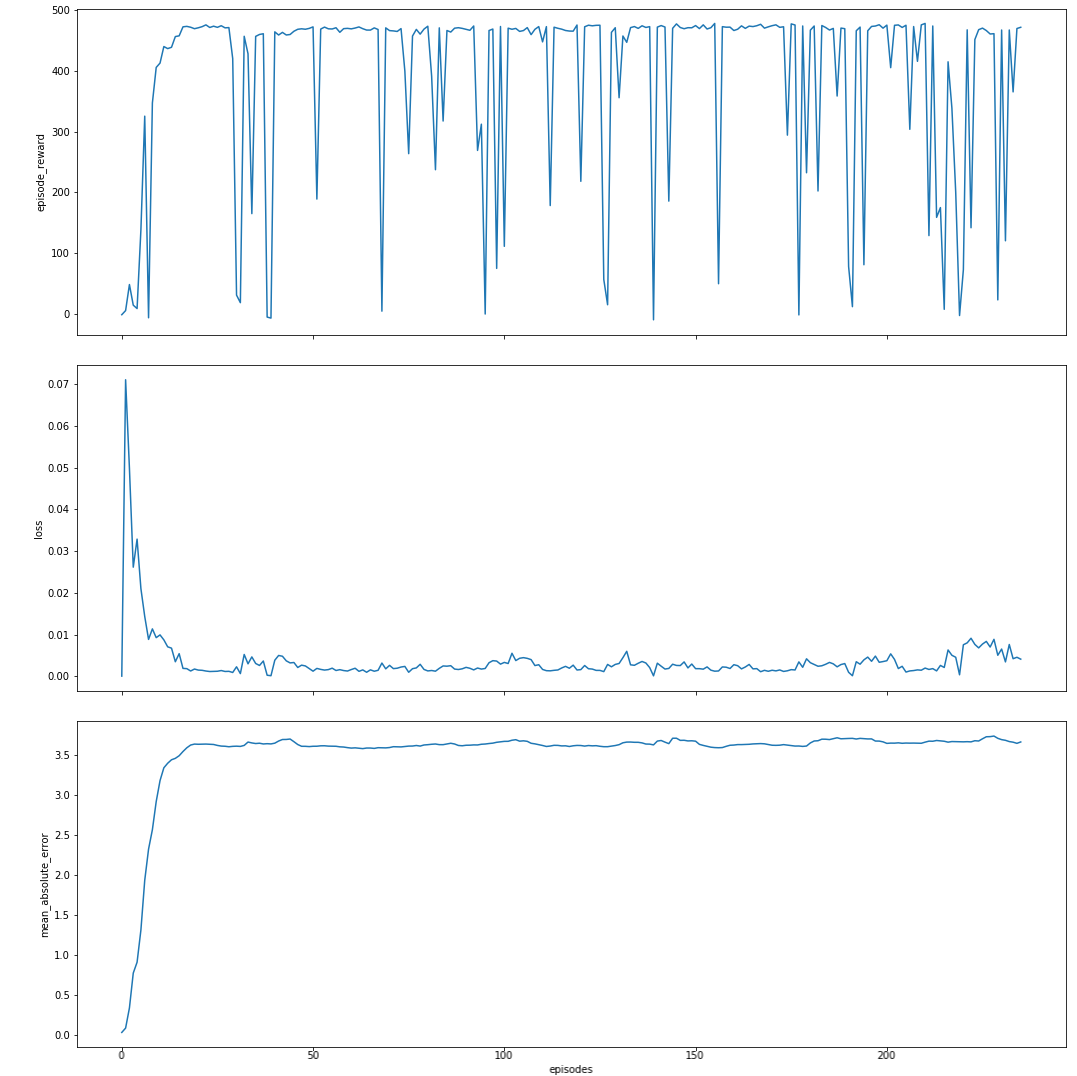
\includegraphics[scale=.4]{test_Exim_v3_2M.png}
    \caption{Graphs for episode reward, loss function and mean absolute error. After training agent for two million steps.}
    \label{fig:dm1}
\end{figure}

\chapter{Discussion \& Conclusions}

\printbibliography[heading=bibintoc] % Print the bibliography (and make it appear in the table of contents)

\appendix 


\chapter{Policy and Value Iteration}\label{app:A}
In this chapter algorithms using dynamic programming for finding optimal value and optimal policy is shown. Based on the material in \parencite{sutton1998reinforcement}.

\section{Value Iteration}
\RestyleAlgo{boxruled}
\LinesNumbered
\begin{algorithm}[H]
 %\KwIn{A MDP i.e.  $(\mathcal{S, A, P, R}, \gamma)$}
 %\KwResult{Returns optimal policy ($\pi_{*}$)}
 \textsf{Initialize $V$ arbitrarily e.g. $V(s) = 0$} \;
 $\Delta \leftarrow 0$ \;
 \While{$\Delta < \theta$ (small positive number)}{
 \ForEach{$s \in \mathcal{S}$}{
 $v \leftarrow V(s)$ \;
 $V(s) \leftarrow \underset{a}{\operatorname{max}} \sum_{s', r}{p(s', r |s, \pi(s))[r + \gamma V(s')]}$ \;
 $\Delta \leftarrow \max(\Delta, |v - V(s)|)$ 
    }
 }
 \KwOut{deterministic policy , $\pi \approx \pi_{*}$ s.t. $\pi (s) = \underset{a}{\operatorname{argmax}} \sum_{s', r}{p(s', r|s,a)[r+\gamma V(s')]}$} 
 \caption{Value iteration}
 \label{alg2}
\end{algorithm}

\section{Policy Iteration}
\RestyleAlgo{boxruled}
\LinesNumbered
\begin{algorithm}[H]
 %\KwIn{A MDP i.e.  $(\mathcal{S, A, P, R}, \gamma)$}
 %\KwResult{Returns optimal policy ($\pi_{*}$)}
 \textsf{1. Initialize} \;
 $V(s) \in \mathbb{R}$ and  $\pi(s) \forall s\in \mathcal{S} $ \;
 $\Delta \leftarrow 0$ \;
 \textsf{2. Policy Evaluation}\;
 \While{$\Delta < \theta$ (small positive number)}{
 \ForEach{$s \in \mathcal{S}$}{
 $v \leftarrow V(s)$ \;
 $V(s) \leftarrow \sum_{s', r}{p(s', r |s, \pi(s))[r + \gamma V(s')]}$ \;
 $\Delta \leftarrow \max(\Delta, |v - V(s)|)$ 
    }
 }
 
 \textsf{3. Policy Improvement}\;
 
 $policy\_stable \leftarrow true$ \;
 \While{$not$ $policy\_stable$)}{
 \ForEach{$s \in \mathcal{S}$}{
 $old\_action \leftarrow \pi(s)$ \;
 $\pi(s) \leftarrow \underset{a}{\operatorname{argmax}} \sum_{s', r}{p(s', r|s,a)[r+\gamma V(s')]}$ \;
 
 \lIf{$old\_action \neq \pi(s)$} {$policy\_stable \leftarrow false$} 
 
  }
  \lIf{$policy\_stable$} {stop} \lElse{go to 2} 
 }
 
 \Return $V \approx v_{*}$ and $\pi \approx \pi_{*}$ \;
 \caption{Policy iteration}
 \label{alg1}
\end{algorithm}

\end{document}
